%!TEX root = forallxyyc.tex

\part{Lógica Modal}
\label{ch.ML}
\addtocontents{toc}{\protect\mbox{}\protect\hrulefill\par}

%\usepackage{gensymb}
%\input{fitch1.sty}

\chapter{Introduzindo a  Lógica Modal}
\label{Intro}


A lógica modal (LM) é a lógica que trata de modalidades, maneiras pelas quais uma afirmação pode ser verdadeira. As duas modalidades mais conhecidas são   \emph{Necessidade} e \emph{Possibilidade}. Uma afirmação pode ser verdadeira, mas também pode ser necessariamente verdadeira (verdadeira não importando como o mundo possa ser). Por exemplo, verdades lógicas não são apenas verdadeiras por causa de alguma característica acidental do mundo, mas verdadeiras em qualquer circunstância. Uma dada afirmação pode não ser realmente verdadeira, mas pode ter sido verdadeira. 
Usamos o operador modal $\ebox$ para expressar \emph{necessidade} e $\ediamond$ para expressar \emph{possibilidade}. Assim, você pode ler $\ebox \metav{A}$ como \emph{é necessariamente o caso que} $\metav{A}$, e $\ediamond \metav{A}$ como \emph{é possivelmente o caso que} $\metav{A}$.

Existem muitos tipos diferentes de necessidade e possibilidade. Por exemplo, é    \emph{humanamente impossível} correr a 200 km/h. Dado o tipo de criaturas que somos, nenhum ser humano pode fazer isso. Mas, ainda assim, não é \emph{fisicamente impossível} correr tão rápido. Ainda não temos a tecnologia para fazer isso, mas certamente é fisicamente possível trocar minhas pernas biológicas por pernas robóticas que possam funcionar a 200 km/h. Por outro lado, é fisicamente impossível correr a uma velocidade maior que a da luz, pois isso iria contra as leis da física. Entretanto, isso não é \emph{logicamente} impossível, pois não é uma contradição imaginar que as leis da física possam ser diferentes e que possam permitir que os objetos se movam mais rápido que a luz.

Com que tipos de modalidade a LM lida? \emph{Todos eles}! A LM é uma ferramenta muito flexível. Começamos com um conjunto básico de regras que regem os operadores modais $\ebox$ e $\ediamond$. Em seguida, adicionamos mais regras para adequar qualquer tipo de modalidade em que estamos interessados. Na verdade, a LM é tão flexível que nem precisamos pensar sempre em $\ebox$ e $\ediamond$ como expressando \emph{necessidade} e \emph{possibilidade} respectivamente. Em vez disso, podemos ler $\ebox$ como expressando \emph{demonstrabilidade}, de modo que $\ebox\metav{A}$ significa   \emph{é demonstrável que} $\metav{A}$, e $\ediamond\metav{A}$ significa \emph{não é refutável que} $\metav{A}$. Da mesma forma, podemos interpretar $\ebox\metav{A}$ como significando $S$ \emph{sabe que  $\metav{A}$} ou $S$ \emph{acredita que $\metav{A}$}, e $\ediamond \metav{A}$ significando que $\metav{A}$ é concebível a $S$. Ou ainda, podemos ler $\ebox$ como expressando \emph{obrigação moral}. Nesse caso, $\ebox \metav{A}$ significa \emph{é moralmente obrigatório que} $\metav{A}$ e $\ediamond \metav{A}$ significa \emph{é moralmente permissível que} $\metav{A}$. Tudo o que precisaríamos fazer é elaborar as regras corretas para essas diferentes leituras de $\ebox$ e $\ediamond$.

Chamamos de sentença modal uma sentença que inclui algum dos operadores modais   $\ebox$ ou $\ediamond$. Cada um dos diferentes modos de interpretar $\ebox$ e $\ediamond$ que mencionamos (necessidade, conhecimento, obrigação moral,...) leva a um  grupo diferente de sentenças que serão classificadas como teoremas ou logicamente válidas. Por exemplo, se $\ebox$ é interpretado como necessidade, a sentença `$\ebox A \eif A$' pode expressar `se $A$ é necessária, é verdadeira'.
  Sob essa  interpretação,  `$\ebox A \eif A$' é válida: todas as afirmações necessárias são verdadeiras aconteça o que acontecer, então são verdadeiras no mundo real. No entanto, quando   $\ebox$  é interpretado como `acredita-se que' ou `é moralmente obrigatório que',  a sentença 
  `$\ebox A \eif A$' não é válida: podemos acreditar em proposições falsas. Nem toda obrigação moral é uma proposição verdadeira. Por exemplo, a sentença ‘Todo assassino enfrentará à justiça’ é uma obrigação moral que, infelizmente, não é verdadeira.

Vamos apresentar diferentes tipos de sistemas da LM, a saber, os sistemas  \mlK, \mlT, \mlSfour{} e \mlSfive.  Eles diferem nas regras de derivação permitidas e na semântica que usaremos para definir nossas noções lógicas.  \mlK{} é o sistema  básico, pois tudo o que é válido ou provado em \mlK{} também pode ser provado nos outros sistemas. 
Veremos que a sentença  `$\ebox A \eif A$'   não é provada em \mlK, mas sim em  \mlT. Isto significa que o sistema \mlT{} é mais apropriado quando se trata de necessidade, porém menos apropriado quando se trata de crença ou obrigação.
O  sistema  \mlSfive,  por sua vez, é considerado como o sistema que melhor  captura os conceitos de possibilidade e necessidade lógica. Além disso, do ponto de vista dedutivo,  \mlSfive{} é o sistema mais forte entre eles.

 

\section{A linguagem da LM}
\label{TFLtoML}

Para poder usar a lógica modal temos que adquirir duas habilidades: precisamos saber fazer provas e precisamos saber construir interpretações. Antes disso, porém, precisamos entender a gramática da LM e saber reconhecer as sentenças corretas de sua linguagem.

A linguagem da LM é uma extensão da LVF. Tem um estoque infinito de \emph{letras sentenciais} (sentenças atômicas); os conectivos lógicos $\enot$, $\eand$,  $\eor$,    $\eif$  e $\eiff$; além dos  operadores modais  $\ebox$ e $\ediamond$.

Se ao invés da LVF tivéssemos estendido a LPO com os operadores modais  $\ebox$ e $\ediamond$, obteríamos um outro conjunto de sistemas modais conhecido como LMQ - Lógica Modal Quantificada. A LMQ é muito mais poderosa do que a LM, mas também é muito, muito mais complicada. Assim,  vamos manter as coisas simples e começar com uma extensão da LVF. 

As regras de construção de  sentenças da LM são todas as da LVF mais duas novas regras para os operadores modais. Assim, temos a seguinte definição formal para uma sentença da LM:
 
 \factoidbox{
\begin{itemize}
	\item[(1)]Toda letra sentencial é uma sentença. 
	\item[(2)]Se $\metav{A}$ é uma sentença, então $\enot\metav{A}$ é uma sentença. 
	\item[(3)]Se $\metav{A}$ e $\metav{B}$ são sentenças, então $(\metav{A}\eand\metav{B})$ é uma sentença.
	\item[(4)]Se $\metav{A}$ e $\metav{B}$ são sentenças, então $(\metav{A}\eor\metav{B})$ é uma sentença.
	\item[(5)]Se $\metav{A}$ e $\metav{B}$ são sentenças, então $(\metav{A}\eif\metav{B})$ é uma sentença.
	\item[(6)]Se $\metav{A}$ e $\metav{B}$ são sentenças, então $(\metav{A}\eiff\metav{B})$ é uma sentença.
	\item[(7)]Se $\metav{A}$ é uma sentença, então $\ebox\metav{A}$ é uma sentença.
	\item[(8)]Se $\metav{A}$ é uma sentença, então $\ediamond\metav{A}$ é uma sentença.
	\item[(9)]Nada além do estabelecido por essas cláusulas é uma sentença. 
\end{itemize}    }
Aqui estão alguns exemplos de sentenças  da LM:
 
 \begin{align*}
			& A \\
			& P\eor Q \\
			& \ebox A \\
			& \ediamond C\eor \ebox D \\
			& \enot\ebox(C\eor \ebox D) \\
			& \ebox\ediamond (S\eand (Z\eiff (\ebox W \eor \ediamond Q))) \\
			& \ \ \vdots
	\end{align*}
 
   
%%%%%%%% ========    chapter{Dedução natural para a LM} ===========================
\chapter{Dedução natural para a LM}
\label{Proof}

Na Parte~\ref{ch.NDTFL}  apresentamos um sistema em dedução natural para a LVF no qual explicitamos as regras de inferência que regem os conetivos lógicos da  LVF.  Agora, sabendo que a linguagem da LM é uma extensão da LVF,  que além dos conectivos lógicos tem os operadores modais   $\ebox$ e $\ediamond$,  precisamos especificar as regras de inferência para tais operadores modais. Ora, é exatamente isso o que faremos neste capítulo. Vamos apresentar os sistemas em dedução  natural  para as lógicas modais  \mlK, \mlT, \mlSfour{} e \mlSfive.

Como  antes,  usaremos `$\proves$' para expressar dedutibilidade. Entretanto, será útil adicionar um índice ao símbolo  `$\proves$' para indicar em qual sistema modal estamos trabalhando. Assim, por exemplo, se quisermos dizer que podemos provar $\metav{C}$ a partir de $\metav{A}_1,\metav{A}_2, \dots \metav{A}_n$ \emph{no sistema}~\mlK, escrevemos: $\metav{A}_1,\metav{A}_2, \dots \metav{A}_n \proves_\mlK \metav{C}$.

Os sistemas em dedução natural para as lógicas modais \mlK, \mlT, \mlSfour{} e \mlSfive{} têm algumas peculiaridades que gostaríamos de chamar atenção. Além de novas regras básicas para o operador modal \ebox{}, eles têm um tipo especial de subprova. 

 Esse  tipo especial de subprova, que chamaremos de  \emph{subprova estrita}, parece uma subprova comum, exceto que tem um~\ebox{} em sua linha de suposição em vez de uma fórmula. Ela nos permite provar coisas e raciocinar sobre possibilidades alternativas. 
 O que podemos provar dentro de uma subprova estrita vale para qualquer possibilidade alternativa, em particular, nas possibilidades alternativas onde as suposições em vigor em nossa prova podem não valer. Em uma subprova estrita todas as suposições param de valer, e não é permitido citar nenhuma linha fora da subprova estrita, com exceção daquelas linhas explicitamente autorizadas por certas regras modais.

Cada sistema modal tem um tipo especial de regra, cujo papel principal é determinar explicitamente o que será permito inserir dentro de uma subprova estrita. Por exemplo, a regra R$\mlK$ vai reger as subprovas estritas do sistema \mlK, a regra R$\mathbf{4}$ vai reger as subprovas  estritas do sistema \mlSfour{} e a regra R$\mathbf{5}$ vai reger as subprovas estritas do sistema \mlSfive{}. 

 Outro fato importante a ressaltar é que a regra de introdução do ~\ebox{} (\ebox I) não é a mesma para todos os sistemas. Embora elas tenham a mesma estrutura, elas diferem quanto às suas restrições. Isso será melhor detalhado nas seções seguintes. 




%%%%  ============  \section{Sistema K}   ===================

\section{Sistema \mlK}
\label{K}

Começamos com um sistema modal particularmente simples, chamado \mlK{} em homenagem ao filósofo e lógico Saul Kripke. O sistema \mlK{} tem todas as regras de dedução natural da  LVF, mais duas novas regras básicas para o operador modal \ebox{}: a regra R$\mlK$  e  a regra de introdução  do ~\ebox{} (\ebox I).

 A regra R$\mlK$ permite introduzir uma sentença $\metav{A}$ em uma subprova estrita, quando $\ebox \metav{A}$ ocorre fora desta subprova. Assumir que uma sentença $\metav{A}$ é necessária (assumir $\ebox\metav{A}$) equivale a assumir $\metav{A}$ em todas as situações alternativas possíveis. É essa ideia que a regra R$\mlK$ descrita a seguir busca expressar:

\factoidbox{
	\[\begin{nd}
			\have[m]{m}{\ebox\metav{A}}
			\open
			\hypo[\ ]{o}{\ebox}
			\have[n]{n}{\metav{A}}\rk{m}
			\close
		\end{nd}\]
		 A linha citada na regra R$\mlK$ (a linha $m$) tem que ocorrer \emph{fora} da subprova estrita que contém a linha em que a regra R$\mlK$  é aplicada (a linha $n$). Além disso, se a subprova estrita que contém a linha $n$ estiver aninhada em outra subprova estrita, a linha $m$, citada, não pode estar fora desta subprova aninhadora. 
		}

A restrição da regra R$\mlK$  é mesmo um pouco confusa, mas sua ideia geral é simples. O que ela faz é evitar que a regra R$\mlK$  seja aplicada em uma situação como a exemplificada abaixo.

\[\begin{nd}
	\have{1}{\ebox\metav{A}}
	\open
	\hypo{2}{\ebox}
	\open
	\hypo{3}{\ebox}
	\have{4}{\metav{A}}\by{uso incorreto de $RK$}{1}
\close\close
\end{nd}\]

Este é um uso ilegítimo da regra porque a linha $4$, onde a regra R$\mlK$ foi aplicada, está em uma subprova estrita (linhas $3-4$) aninhada em outra subprova estrita (linhas $2-4$). Então, de acordo com a restrição, a sentença citada deveria estar fora da subprova das linhas $3-4$, mas dentro da subprova das linhas $2-4$. A ideia é evitar que se cite sentenças separadas por mais de um nível de aninhamento de subprovas estritas.
 

A regra \ebox I, por sua vez, nos permite derivar uma sentença $\ebox \metav{A}$ se pudermos derivar $\metav{A}$ dentro de uma subprova estrita. Esse é  nosso método fundamental para introduzir \ebox{} nas provas. A ideia básica é bastante simples: se $\metav{A}$ é um teorema, então  $\ebox \metav{A}$ deve ser um teorema também.  Lembre-se de que se $\metav{A}$ é um teorema, então é possível apresentar uma prova de $\metav{A}$ que não parte de nenhuma premissa, ou seja, na qual não há nenhuma suposição não descartada.

Suponha que queremos provar `$\ebox(A\eif A)$'. A primeira coisa que precisamos fazer é provar que `$A\eif A$' é um teorema. Isso você já sabe como fazer na LVF,  simplesmente apresentando uma prova de `$A\eif A$'  como esta:
\[
	\begin{nd}
		\open
		\hypo{1}{A}
		\have{2}{A}\by{R}{1}
		\close
		\have{3}{A\eif A}\ci{1-2}
	\end{nd}
\]
Claramente, a prova de `$A \eif A$' não faz uso de nenhuma suposição não descartada.  Assim, para aplicar a regra \ebox I, precisamos apenas inserir essa prova dentro de uma subprova estrita, como segue:


\[\begin{nd}
		\open
		\hypo{1}{\ebox}
		\open
		\hypo{2}{A}
		\have{3}{A}\by{R}{2}
		\close
		\have{4}{A\eif A}\ci{2-3}
		\close
		\have{5}{\ebox(A\eif A)}\boxi{1-4}
	\end{nd}\]


A regra \ebox I, de introdução do \ebox, pode então ser assim apresentada:

\factoidbox{
	\[\begin{nd}
			\open
			\hypo[m]{m}{\ebox}
			\have[n]{n}{\metav{A}}
			\close
			\have[\,]{o}{\ebox\metav{A}}\boxi{m-n}
		\end{nd}\]
	Nenhuma linha da subprova estrita pode citar qualquer linha fora da subprova estrita, com exceção daquelas linhas  justificadas pela regra R$\mlK$.
}

Não é demais enfatizar a importância da restrição de aplicação desta regra. Salvo as linhas citadas por aplicações da regra  R$\mlK$,  nenhuma linha externa à subprova estrita pode ser citada nas justificativas das regras das linhas internas à subprova. Essa restrição é essencial, caso contrário, obteríamos resultados terríveis. Por exemplo, poderíamos produzir a seguinte prova para justificar  $A\therefore \ebox A$:
\[\begin{nd}
		\hypo{1}{A}
		\open
		\hypo{2}{\ebox}
		\have{3}{A}\by{R}{1}
		\close
		\have{4}{\ebox A}\by{uso incorreto de $\ebox$I }{2-3}
	\end{nd}
\]
Essa não é uma prova legítima. Como uma linha interna da subprova estrita (a linha 3) cita uma linha externa (a linha 1), então a restrição de aplicação da regra \ebox I não é satisfeita e, portanto, sua aplicação na linha 4 é ilegítima.


 
Vejamos agora um exemplo com aplicações corretas das regras \ebox I e R$\mlK$. 
\[
	\begin{nd}
		\hypo{1}{\ebox A}
		\hypo{2}{\ebox B}
		\open
		\hypo{3}{\ebox}
		\have{4}{A}\rk{1}
		\have{5}{B}\rk{2}
		\have{6}{A \eand B}\ai{4,5}
		\close
		\have{6}{\ebox(A \land B)}\boxi{3-6}
	\end{nd}
\]


Também podemos misturar subprovas regulares e subprovas estritas, como podemos ver na seguinte prova de  $\ebox (A \eif B) \proves_\mlK  \ebox A \eif \ebox B$. Repare que em $3-6$ há uma subprova estrita, mas em $2-7$ a subprova é regular.


\[\begin{nd}
		\hypo{1}{\ebox (A \eif B)}
		\open
		\hypo{2}{\ebox A}
		\open
		\hypo{3}{\ebox}
		\have{4}{A}\rk{2}
		\have{5}{A \eif B}\rk{1}
		\have{6}{B}\ce{4,5}
		\close
		\have{7}{\ebox B}\boxi{3-6}
		\close
		\have{8}{\ebox A \eif \ebox B} \ci{2-7}
	\end{nd}\]
Essa é chamada  de \emph{regra de distribuição}, porque nos diz que $\ebox$ `distribui' sobre $\eif$.

As regras \ebox I e R$\mlK$ parecem bastante simples e, de fato, \mlK{} é um sistema muito simples! Mas \mlK{} é mais poderoso do que você pode imaginar. Você também pode  provar outras coisas nele.
   

%%%%  \section{Possibilidade}

\section{Possibilidade}
\label{possibility}

Na seção anterior, vimos todas as regras básicas para \mlK. Mas você deve ter notado que todas essas regras eram sobre necessidade,  $\ebox$, e nenhuma delas era sobre possibilidade, $\ediamond$. Isso não é um problema uma vez que podemos \emph{definir} possibilidade em termos de necessidade:
\factoidbox{
$\ediamond\metav{A}=_{df} \enot \ebox\enot \metav{A}$
}
Em outras palavras, dizer que $\metav{A}$ é \emph{possivelmente verdadeira}, é dizer que $\metav{A}$   \emph{não é necessariamente falsa}. Como resultado, não é realmente essencial adicionar um símbolo novo para possibilidade  no sistema \mlK. Ainda assim, o sistema será \emph{muito mais} fácil de usar se o fizermos. Por isso, adicionaremos as seguintes regras de definição:
\factoidbox{
	\[\begin{nd}
			\have[m]{m}{\enot\ebox\enot \metav{A}}
			\have[\, ]{n}{\ediamond \metav{A}}\diadf{m}
		\end{nd}
	\]
	\[\begin{nd}
			\have[m]{m}{\ediamond \metav{A}}
			\have[\, ]{n}{\enot\ebox\enot \metav{A}}\diadf{m}
		\end{nd}\]
}
É importante ressaltar que essas regras registram apenas a maneira como  o operador $\ediamond$  é definido em termos de $\ebox$ e, do ponto de vista dedutivo, elas não representam nenhuma adição real ao sistema \mlK. Entretanto, além dessas,  será útil adicionar outras \emph{regras de conversão modal} que nos fornecem maneiras  diferentes de alternar  $\ebox$  e $\ediamond$:
 

\factoidbox{
	\[\begin{nd}
			\have[m]{m}{\enot\ebox \metav{A}}
			\have[\, ]{n}{\ediamond \enot\metav{A}}\mc{m}
		\end{nd}
	\]
	\[\begin{nd}
			\have[m]{m}{\ediamond \enot \metav{A}}
			\have[\, ]{n}{\enot\ebox \metav{A}}\mc{m}
		\end{nd}\]
	\[\begin{nd}
			\have[m]{m}{\enot\ediamond \metav{A}}
			\have[\, ]{n}{\ebox \enot\metav{A}}\mc{m}
		\end{nd}\]
	\[\begin{nd}
			\have[m]{m}{\ebox\enot \metav{A}}
			\have[\, ]{n}{\enot\ediamond\metav{A}}\mc{m}
		\end{nd}\]
}
Todas essas regras de conversão modal podem ser derivadas das regras básicas de \mlK, usando a  definição de $\ediamond$ apresentada acima. 

No sistema   \mlK, escolhemos $\ebox$ como nosso símbolo modal primitivo e, em seguida, definimos $\ediamond$ em termos dele. Mas, poderíamos ter começado com $\ediamond$ como símbolo  primitivo, e então definido $\ebox$ como segue: $\ebox\metav{A} =_{df} \enot \ediamond \enot \metav{A}$. 
Assim,  não há nenhum sentido em que a necessidade seja de alguma forma mais \emph{fundamental} do que a possibilidade. A necessidade é tão fundamental quanto a possibilidade em contextos modais.

%%%%%\==============  section{Sistema T}  ================

\section{Sistema \mlT}
\label{T}

O sistema  \mlK{}   é um sistema modal muito simples e  tão fraco que nem mesmo permite que você prove uma sentença $\metav{A}$  a partir de $\ebox\metav{A}$.  Mas se estivermos pensando em $\ebox$ como expressando \emph{necessidade}, deveríamos ser capazes de fazer esta inferência: se $\metav{A}$ é \emph{necessariamente verdadeira}, então ela certamente deve ser \emph{verdadeira}!

Isso nos leva a um novo sistema modal, \mlT, que obtemos adicionando  ao sistema \mlK{}  a seguinte regra de eliminação do $\ebox$ ($\ebox$E), também conhecida como  R\mlT{}:
\factoidbox{
	\[\begin{nd}
			\have[m]{m}{\ebox \metav{A}}
			\have[n]{n}{\metav{A}}\boxe{m}
		\end{nd}\]
	A linha $n$ na qual a regra \ebox E é aplicada  \emph{não deve} estar em uma subprova estrita que começa após a linha~$m$.
}

A restrição da regra \ebox E é, de certa forma, oposta à restrição em R$\mlK$. 
O que esta restrição busca garantir é que se a regra \ebox E for aplicada em uma subprova estrita, então a regra citada tem que estar na mesma subprova estrita (e no mesmo nível de aninhamento, caso haja subprovas estritas aninhadas dentro de subprovas estritas).

Com a inclusão da regra \ebox E, podemos provar coisas em \mlT{} que não poderíamos provar em \mlK, como `$\ebox A \eif A$'.

%%%%%\==============section{Sistema S4}  ================
\section{Sistema \mlSfour}
\label{S4}

Vimos que no sistema \mlT{} é permitido retirar as caixas de necessidade de uma sentença: de $\ebox \metav{A}$, você pode inferir $\metav{A}$. Mas, e se quiséssemos adicionar caixas extras?  Ou seja, podemos ir de $\ebox\metav{A}$ para $\ebox\ebox\metav{A}$? 

Bem, isso pode ser feito no sistema \mlT{} desde que $\metav{A}$ seja um teorema. Porque do mesmo modo que você pode colocar a prova de $\metav{A}$ dentro de uma subprova estrita e aplicar a regra \ebox I para concluir $\ebox\metav{A}$; você pode repetir este processo quantas vezes quiser. Ou seja, você pode colocar a prova de $\metav{A}$ em uma subprova estrita aninhada em outra subprova estrita e com duas aplicações da regra \ebox I concluir $\ebox\ebox \metav{A}$.
Por exemplo, podemos provar `$\ebox\ebox (P\eif P)$' da seguinte forma: 
 

\[
	\begin{nd}
		\open
		\hypo{1}{\ebox}
		\open
		\hypo{2}{\ebox}
		\open
		\hypo{3}{P}
		\have{4}{P}\by{R}{3}
		\close
		\have{5}{P\eif P}\ci{3-4}
		\close
		\have{6}{\ebox(P\eif P)}\boxi{2-5}
		\close
		\have{7}{\ebox\ebox(P\eif P)}\boxi{1-6}
	\end{nd}
\]

Veja que colocamos a prova do teorema `$P\eif P$' dentro de duas subprovas estritas uma aninhada na outra e ao final aplicamos a regra \ebox I duas vezes.


Mas essa estratégia de obter $\ebox\ebox\metav{A}$ a partir de $\ebox\metav{A}$ no sistema \mlT{} só funciona quando $\metav{A}$ é um teorema. Se, por exemplo, $\ebox\metav{A}$ tivesse sido assumida como uma hipótese, não poderíamos usar a regra \ebox I para obter $\ebox\ebox\metav{A}$ pois a restrição dessa regra seria desrespeitada. Ou ainda, se tivéssemos usado a regra R$\mlK$ na subprova estrita onde provamos $\metav{A}$, não poderíamos colocar uma subprova estrita aninhada dentro de outra para obter $\ebox\ebox\metav{A}$ como fizemos no exemplo acima, porque a restrição para a aplicação da regra R$\mlK$ seria violada.

O único caso em que o sistema \mlT{} permite obter $\ebox\ebox\metav{A}$ a partir de   $\ebox\metav{A}$ é mesmo quando $\metav{A}$ é um teorema da LVF. E isso pode muito bem lhe parecer uma limitação de \mlT{}, pelo menos se estivermos lendo $\ebox$ como expressando necessidade. Nesse caso parece intuitivo que se $\metav{A}$ for mesmo necessariamente verdadeira, então $\metav{A}$ não poderia não ser necessariamente verdadeira. E se você lembrar de nossa definição de possibilidade, dizer que não é possível que $\metav{A}$ não seja necessariamente verdadeira é o mesmo que dizer que é necessariamente o caso que $\metav{A}$ é necessariamente verdadeira. Trocando em miúdos, temos uma certa intuição de que onde vale $\ebox\metav{A}$ deveria valer também $\ebox\ebox\metav{A}$.

Para que a LM incorpore esta intuição precisamos de mais um sistema, o sistema  \mlSfour{},  que obtemos expandindo sistema  \mlT{}, da seguinte forma: vamos adicionar uma nova regra modal,  a regra R$\mathbf{4}$,  e alterar  as restrições da regra~\ebox I, para torná-la mais permissível.

A regra R$\mathbf{4}$ desempenha um papel semelhante ao da regra R$\mlK$  no sistema \mlK{}  com respeito às subprovas estritas.  Aqui no sistema \mlSfour{}, a regra R$\mathbf{4}$  permite introduzir uma sentença $\ebox \metav{A}$ dentro de uma subprova estrita,  com as condições descritas abaixo:
 
\factoidbox{
	\[\begin{nd}
			\have[m]{m}{\ebox\metav{A}}
			\open
			\hypo[\ ]{k}{\ebox}
			\have[n]{n}{\ebox\metav{A}}\rfour{m}
			\close
		\end{nd}
	\]
	A linha citada na regra R$\mathbf{4}$ (a linha $m$) tem que ocorrer fora da subprova estrita que contém a linha em que a regra R$\mathbf{4}$ é aplicada (a linha $n$). Além disso, se a subprova estrita que contém a linha $n$ estiver aninhada em outra subprova estrita, a linha $m$, citada, não pode estar fora desta subprova aninhadora.

}


A regra R$\mathbf{4}$ é quase idêntica à regra R$\mlK$: as duas nos dão autorizações excepcionais para colocar sentenças dentro de subprovas estritas; as duas exigem a citação de uma sentença com a forma $\ebox \metav{A}$; e as duas têm exatamente a mesma restrição de aplicação. A única diferença entre elas é que partindo de $\ebox \metav{A}$ a regra R$\mlK$ autoriza colocar $\metav{A}$ dentro de uma subprova estrita e a regra R$\mathbf{4}$ autoriza colocar a própria $\ebox \metav{A}$ dentro de uma subprova estrita.

Vimos na Seção \ref{K} 
 que a restrição da regra  \ebox I do sistema \mlK{}  impõe que,  salvo as linhas citadas por aplicações da regra R$\mlK$, nenhuma linha externa à subprova estrita pode ser citada nas justificativas das regras das linhas internas à subprova.  Mas, agora no sistema \mlSfour{} temos uma uma nova regra, a regra R$\mathbf{4}$,  que  autoriza colocar outras sentenças  dentro de uma subprova estrita (sentenças da forma $\ebox\metav{A}$ ).  A regra \ebox I, de introdução do \ebox, para  o sistema  \mlSfour{}  pode então ser assim apresentada:


\factoidbox{
	\[\begin{nd}
			\open
			\hypo[m]{m}{\ebox}
			\have[n]{n}{\metav{A}}
			\close
			\have[\,]{o}{\ebox\metav{A}}\boxi{m-n}
		\end{nd}\]
	Nenhuma linha da subprova estrita pode citar qualquer linha fora da subprova estrita, com exceção daquelas linhas  justificadas pelas regras R$\mlK$ ou  R$\mathbf{4}$.
}


Agora podemos provar ainda mais resultados. Por exemplo, $\proves_\mlSfour \ebox A  \eif \ebox\ebox A$:

\[\begin{nd}
	\open
	\hypo{1}{\ebox A}
	\open
	\hypo{2}{\ebox}
	\have{3}{\ebox A}\rfour{1}
	\close
	\have{4}{\ebox\ebox A}\boxi{2-3}
	\close
	\have{5}{\ebox A \eif \ebox\ebox A}\ci{1-6}
\end{nd}\]
Da mesma forma, podemos provar `$\ediamond\ediamond A \eif \ediamond A$'. Isso nos mostra que, além ser possível \emph{adicionar}  \emph{caixas extras}, no sistema \mlSfour{} também podemos \emph{excluir losangos extras}: de $\ediamond\ediamond \metav{A}$, você sempre pode inferir $\ediamond\metav{A}$.


%%%%%\==============section{Sistema S5}  ================
\section{Sistema \mlSfive}
\label{S5}

No sistema  \mlSfour{} sempre podemos adicionar uma caixa na frente de outra caixa, mas não podemos adicionar automaticamente uma caixa na frente de um  \emph{losango}. Ou seja,  \mlSfour{}  geralmente não permite a inferência de $\ebox\ediamond\metav{A}$ a partir de  $\ediamond\metav{A}$. Isso pode lhe parecer uma lacuna, pelo menos se você estiver lendo $\ebox$ e $\ediamond$ como expressando \emph{necessidade} e \emph{possibilidade} respectivamente. 
Parece intuitivo que se $\metav{A}$ é possivelmente verdadeira, então não poderia deixar de ser possivelmente verdadeira. Ou seja, se $\metav{A}$ é possivelmente verdadeira ($\ediamond\metav{A}$), então necessariamente $\metav{A}$ é possivelmente verdadeira ($\ebox\ediamond\metav{A}$). O sistema modal \mlSfive{} nos permite incluir esta intuição na LM. Ele é obtido adicionando-se a seguinte regra ao sistema \mlSfour:

\factoidbox{
	\[\begin{nd}
			\have[m]{m}{\enot \ebox\metav{A}}
			\open
			\hypo[\ ]{k}{\ebox}
			\have[n]{n}{\enot\ebox\metav{A}}\rfive{m}
			\close
	\end{nd}\]
	A linha citada na regra R$\mathbf{5}$ (a linha $m$) tem que ocorrer fora da subprova estrita que contém a linha em que a regra R$\mathbf{5}$ é aplicada (a linha $n$). Além disso, se a subprova estrita que contém a linha $n$ estiver aninhada em outra subprova estrita, a linha $m$, citada, não pode estar fora desta subprova aninhadora..
}

A regra R$\mathbf{5}$ é muito semelhante à regra R$\mathbf{4}$. Ambas têm o mesmo aspecto geral e a mesma restrição. A única diferença entre elas é a forma da sentença que elas autorizam entrar em uma subprova estrita. R$\mathbf{4}$ autoriza a entrada de sentenças com a forma $\ebox \metav{A}$ e R$\mathbf{5}$ autoriza sentenças com a forma $\enot\ebox\metav{A}$.

Aqui no sistema \mlSfive{}, também precisamos adequar a regra de introdução do \ebox,  modificando a sua restrição para permitir também citações da regra R$\mathbf{5}$ dentro da subprova estrita explícita na regra \ebox I, como veremos abaixo: 

\factoidbox{
	\[\begin{nd}
			\open
			\hypo[m]{m}{\ebox}
			\have[n]{n}{\metav{A}}
			\close
			\have[\,]{o}{\ebox\metav{A}}\boxi{m-n}
		\end{nd}\]
	Nenhuma linha da subprova estrita pode citar qualquer linha fora da subprova estrita, com exceção daquelas linhas  justificadas pelas regras R$\mlK$, R$\mathbf{4}$ ou R$\mathbf{5}$ .
}



Agora com a regra R$\mathbf{5}$ podemos adicionar uma caixa na frente de um losango, ou seja, podemos mostrar que  $\ediamond A\proves_\mlSfive  \ebox\ediamond A$:
\[\begin{nd}
\hypo{1}{\ediamond A}
\have{2}{\enot\ebox\enot A}\by{Def\ediamond}{1}
\open
\hypo{3}{\ebox}
\have{4}{\enot\ebox\enot A}\rfive{2}
\have{5}{\ediamond A}\by{Def\ediamond}{4}
\close
\have{6}{\ebox\ediamond A}\boxi{3-5}
\end{nd}\]


A  regra R$\mathbf{5}$  também  nos permite mostrar que $\ediamond\ebox A\proves_\mlSfive  \ebox A$:
\[\begin{nd}
	\hypo{1}{\ediamond\ebox A}
	\have{2}{\enot\ebox\enot\ebox A}\by{Def\ediamond}{1}
	\open
	\hypo{3}{\enot \ebox A}
	\open
	\hypo{4}{\ebox}
	\have{5}{\enot\ebox A}\rfive{3}
	\close
	\have{6}{\ebox\enot\ebox A}\boxi{4-5}
	\have{7}{\ered}\ne{2,6}
	\close
	\have{8}{\ebox A}\by{IP}{3-7}
\end{nd}\]

Assim, além de adicionar caixas na frente de losangos, também podemos excluir os losangos que estão na frente das caixas.

Obtemos \mlSfive{} apenas adicionando a regra R$\mathbf{5}$  a \mlSfour. Na verdade, poderíamos ter adicionado a regra R$\mathbf{5}$ a \mlT{} sozinha, e deixar de fora a regra R$\mathbf{4}$. Tudo o que podemos provar com a regra R$\mathbf{4}$ também pode ser provado usando \ebox E junto com R$\mathbf{5}$. Por exemplo, aqui está uma prova que mostra $\ebox A \proves_\mlSfive  \ebox\ebox A$ sem usar R$\mathbf{4}$:

\[\begin{nd}
	\hypo{1}{\ebox A}
	\open
	\hypo{2}{\ebox\enot\ebox A}
	\have{3}{\enot\ebox A}\boxe{2}
	\have{4}{\ered}\ne{1,3}
	\close
	\have{5}{\enot\ebox\enot\ebox A}\ni{2-4}
	\open
	\hypo{6}{\ebox}
	\open
	\hypo{7}{\enot\ebox A}
	\open
	\hypo{8}{\ebox}
	\have{9}{\enot\ebox A}\rfive{7}
	\close
	\have{10}{\ebox \enot\ebox A}\boxi{8-9}
	\have{11}{\enot\ebox\enot\ebox A}\rfive{5}
	\have{12}{\ered}\ne{10,11}
	\close
	\have{13}{\ebox A}\ip{7-12}
	\close
	\have{14}{\ebox\ebox A}\boxi{6-13}
\end{nd}\]
Acabamos de ver que o sistema \mlSfive{} é \emph{estritamente mais forte} que \mlSfour, pois há coisas que podem ser provadas em \mlSfive{}, mas não podem em \mlSfour{}  como por exemplo: `$\ediamond\ebox A \eif \ebox A$'.  

O ponto importante sobre \mlSfive{} pode ser colocado assim: se você tiver uma longa sequência de caixas e losangos em qualquer combinação, você pode excluir todos, exceto o último. Por exemplo, a sentença `$\ediamond\ebox\ediamond\ediamond\ebox\ebox\ediamond\ebox A$' pode ser simplificada para   `$\ebox A$' com apenas um operador.

\practiceproblems

\problempart
Forneça provas em \mlK{}  para as quatro seguintes asserções:
\begin{earg}
	\item $\ebox (A\eand B)\proves_\mlK\ebox A \eand \ebox B$
	\item $\ebox A\eand\ebox B\proves_\mlK\ebox( A \eand  B)$
	\item $\ebox A\eor\ebox B\proves_\mlK\ebox( A \eor  B)$
	\item $\ebox (A \eiff B)\proves_\mlK \ebox A \eiff \ebox B$
\end{earg}

\problempart
Forneça provas em \mlK{}  para as quatro seguintes asserções  (sem usar a Conversão Modal!):
\begin{earg}
	\item $\enot\ebox A\proves_\mlK \ediamond \enot A$
	\item $\ediamond\enot A\proves_\mlK\enot \ebox A$
	\item $\enot\ediamond A\proves_\mlK\ebox\enot A$
	\item $\ebox\enot A\proves_\mlK\enot\ediamond A$
\end{earg}

\problempart
Forneça provas  em \mlK{}  para as três seguintes asserções (e agora sinta-se à vontade para usar a Conversão Modal!):
\begin{earg}
	\item $\ebox(A\eif B), \ediamond A \proves_\mlK \ediamond B$
	\item $\ebox A \proves_\mlK \enot\ediamond\enot A$
	\item $\enot\ediamond\enot A \proves_\mlK \ebox A$
\end{earg}

\problempart
Forneça provas em  \mlT{} para as duas seguintes asserções:
\begin{earg}
	\item $P\proves_\mlT\ediamond P$
	\item $\proves_\mlT (A\eand B)\eor(\enot \ebox A\eor\enot\ebox B)$
\end{earg}

\problempart
Forneça provas em  \mlSfour{}  para as três seguintes asserções:
\begin{earg}
	\item $\ebox(\ebox A\eif B), \ebox (\ebox B\eif C), \ebox A \proves_\mlSfour \ebox\ebox C$
	\item $\ebox A \proves_\mlSfour \ebox(\ebox A \eor B)$
	\item $\ediamond \ediamond A \proves_\mlSfour \ediamond A$
\end{earg}

\problempart
Forneça provas em \mlSfive{} para as três seguintes asserções:
\begin{earg}
	\item $\enot\ebox\enot A, \ediamond B\proves_\mlSfive \ebox(\ediamond A \eand \ediamond B)$
	\item $A \proves_\mlSfive  \ebox\ediamond A$
	\item $\ediamond\ediamond A\proves_\mlSfive  \ediamond A$
\end{earg}

%%%% ================= Semântica para  a LM ============
\chapter{Semântica para  a  LM}
\label{Semantics}

Neste capítulo, vamos tratar dos aspectos \emph{semânticos} da Lógica modal.  Inicialmente veremos as circunstâncias sob as quais sentenças modais são consideradas verdadeiras. Em seguida, veremos como avaliar a validade de argumentos envolvendo tais sentenças modais, levando em consideração as peculiaridades dos diversos sistemas  de  dedução natural  apresentados no capítulo anterior. Para dar conta de tudo isso, veremos também  que será necessário  estender os conceitos semânticos da LVF apresentados no Capítulo \ref{s:SemanticConcepts}. 

%%%% =================  Interpretações da LM ============
\section{Interpretações da LM}

A grande ideia por trás da semântica da LM é que as sentenças não são apenas verdadeiras ou falsas e ponto final.  Dizemos que uma  sentença é verdadeira ou falsa em \emph{um dado mundo possível}. Assim,  a mesma sentença pode muito bem ser verdadeira em alguns mundos,  mas falsa em outros. Grosso modo, dizemos que $\ebox \metav{A}$ é verdadeira   se e somente se $\metav{A}$ é verdadeira em \emph{todos} os mundos possíveis, e $\ediamond\metav{A}$ é verdadeira se e somente se  $\metav{A}$ é verdadeira em \emph{algum} mundo.

Precisamos refinar essa ideia e torná-la mais precisa. Para fazer isso,  vamos especificar o que é uma  \emph{interpretação} para a LM. A primeira coisa que você precisa incluir em uma interpretação é uma coleção de \emph{mundos possíveis}. 
Mas, o que exatamente é um mundo possível? A ideia por trás da noção de mundo possível é a mesma que suscita a noção de situação, que vimos no Capítulo \ref{s:Valid}, Seção \ref{ss:Validade}. Um mundo possível é uma alternativa concebível para o mundo. Os fatos que compõem o mundo real poderiam ocorrer diferentemente de como ocorrem. Eu poderia ser canhoto, ter nascido em Cuba, poderia estar nevando agora em Natal, etc. Um mundo possível é uma versão alternativa para o mundo real onde um ou mais fatos são substituídos por outros que não ocorrem, mas que poderiam ocorrer ou ter ocorrido. 
Há uma grande discussão filosófica sobre  essa questão que examinaremos com mais detalhes posteriormente. Agora, no entanto,  não precisamos nos preocupar muito com isso, pois no que diz respeito à lógica formal, os mundos possíveis podem ser o que você quiser. Tudo o que importa é que você forneça a cada interpretação uma coleção não vazia de coisas rotuladas  de  \definepl{possible world}.


Mas como determinar quais sentenças da LM são verdadeiras em quais mundos possíveis? Para fazer isso, precisamos introduzir a noção de uma \emph{função de valoração}. Aqueles que estudaram matemática já estão familiarizados com a ideia geral de função: uma entidade matemática que mapeia argumentos em valores. Isso pode parecer um pouco abstrato, mas alguns exemplos familiares ajudarão. Considere a função $x + 1$. Essa é uma função que recebe um número como argumento e, em seguida, fornece um número como valor. Portanto, se você inserir o número $1$ como um argumento, a função $x + 1$ fornecerá o número $2$ como valor; se você inserir o número  $2$, ela fornecerá $3$; se você inserir o número  $3$, ela fornecerá $4$ \dots{}  No caso da função $x + y$, você deve inserir dois argumentos, se quiser que ela retorne um valor: se você inserir $2$ e $3$ como seus argumentos, ela produzirá $5$; se você inserir os números  $1003$ e $2005$, ela fornecerá como resultado $3008$; e assim por diante.

Dito isso, podemos entender uma função de valoração para a LM como uma função que toma dois argumentos como entrada, uma sentença e um mundo possível, e devolve como saída um valor de verdade (ou V ou F). 
Mais precisamente, se $\nu$   é uma função de valoração  e $w$ é um mundo possível,   $\nu_w(\metav{A})=F$  se e somente se $\metav{A}$ é falsa no mundo $w$ na valoração $\nu$; e $\nu_w(\metav{A})=V$  se e somente se $\metav{A}$  é verdadeira no mundo $w$ na valoração $\nu$.

Você deve se lembrar da LVF, que uma valoração corresponde a uma atribuição arbitrária de $V$ e $F$ para as \emph{letras sentenciais}. Cada linha em uma tabela de verdade representa uma função de valoração diferente. Aí, com os valores de verdade das letras sentenciais definidos, nós conseguimos calcular os valores de verdade das sentenças complexas em cada uma das valorações (linhas da tabela).

Por exemplo, na LVF, para saber se o valor de verdade da sentença `$A\eand B$' é $V$ ou $F$ em uma certa valoração $\nu$, precisamos saber que valores a valoração $\nu$ atribui para as letras sentenciais `$A$' e $B$', e aí calculamos o valor de `$A\eand B$' através da tabela de verdade característica da conjunção. Neste caso, $\nu(A\eand B)=V$ se e somente se $\nu(A)=V$ e $\nu(B)=V$.   

A situação aqui na Lógica Modal (LM) é similar, mas com o acréscimo dos mundos possíveis. 
Enquanto na LVF cada interpretação consiste apenas de uma valoração $\nu$ que atribui um único valor de verdade a uma letra sentencial `$A$', digamos, v(A)=V,   na LM cada interpretação é constituída por uma coleção $W$ de mundos possíveis, e uma valoração $\nu$ que atribui tantos valores de verdade a cada letra sentencial quantos forem os mundos possíveis de $W$. Assim, supondo que há 4 mundos possíveis em $W$, a valoração $\nu$ atribuirá 4 valores de verdade à letra sentencial `$A$', por exemplo: $\nu_{w1}(A)=V$, $\nu_{w2}(A)=F$,  $\nu_{w3}(A)=F$,  $\nu_{w4}(A)=V$. Então, de um ponto de vista estritamente semântico, uma coleção de mundos possíveis não é nada mais que uma coleção de índices para valores de verdade alternativos para as letras sentenciais.

O que descrevemos acima para as sentenças complexas da LVF repete-se em cada um dos mundos possíveis da LM. O valor de verdade de `$A\eand B$' em uma valoração $\nu$  
 ($\nu (A,B)$)  não depende apenas dos valores de verdade de `$A$' e de `$B$' ($\nu (A)$ e $\nu(B)$). 
Depende também de qual mundo possível estamos considerando. Na valoração $\nu$,  `$A$' pode ser verdadeira no mundo $w_1$, mas falsa em $w_2$
  ($\nu_{w_1}(A)=V$ e $\nu_{w_2}(A)=F$). Então o que temos na LM é que para cada mundo possível $w$ e valoração $\nu$, $\nu_w(A\eand B) = V$ se e somente se a $\nu_w(A) = V$ e $\nu_w(A) = V$.

Aqui estão as regras para cada um dos conectivos da LVF que determinam os valores de verdade de sentenças complexas na LM a partir de sentenças mais simples:

\begin{itemize}
	\item[(1)]$\nu_w(\enot\metav{A})=V$ se e somente se $\nu_w(\metav{A})=F$
	\item[(2)]$\nu_w(\metav{A}\eand\metav{B})=V$ se e somente se $\nu_w(\metav{A})=V$ e $\nu_w(\metav{B})=V$
	\item[(3)]$\nu_w(\metav{A}\eor\metav{B})=V$ se e somente se $\nu_w(\metav{A})=V$ ou $\nu_w(\metav{B})=V$
	\item[(4)]$\nu_w(\metav{A}\eif\metav{B})=V$ se e somente se $\nu_w(\metav{A})=F$ ou $\nu_w(\metav{B})=V$
	\item[(5)]$\nu_w(\metav{A}\eiff\metav{B})=V$ se e somente se $\nu_w(\metav{A})=\nu_w(\metav{B})$  
\end{itemize}
 

Até agora, todas essas regras devem parecer muito familiares. Essencialmente, todas elas funcionam exatamente como as tabelas de verdade para a LVF. A única diferença é que na LM as regras das tabelas de verdade repetem-se em cada um dos mundos possíveis.
Mas quais são as regras para os novos operadores modais, $\ebox$ e $\ediamond$? A ideia mais óbvia seria fornecer regras como estas:

\begin{itemize}
	\item[]$\nu_w(\ebox \metav{A})=V$ se e somente se $\forall w' (\nu_{w'}(\metav{A})=V)$
	\item[]$\nu_w(\ediamond \metav{A})=V $ se e somente se $\exists w' (\nu_{w'}(\metav{A})=V)$
\end{itemize}
Essa é apenas a maneira formal sofisticada de escrever a ideia de que $\ebox\metav{A}$ é verdadeira em $w$ apenas no caso de $\metav{A}$ ser verdadeira em \emph{todos} os mundos, e $\ediamond\metav{A}$ é verdadeira em $w$ apenas no caso de $\metav{A}$ ser verdadeira em \emph{algum} mundo.

No entanto, embora essas regras sejam boas e simples, elas acabam não sendo tão úteis quanto gostaríamos. Como mencionamos, a LM deve ser uma ferramenta muito flexível. Pretende ser uma estrutura geral para lidar com muitos tipos diferentes de necessidade. Como resultado, queremos que nossas regras semânticas para  $\ebox$ e $\ediamond$ sejam um pouco menos rígidas. Podemos fazer isso introduzindo outra ideia nova: \emph{ relações de acessibilidade}.

Uma relação de acessibilidade, $R$, é uma relação entre mundos possíveis. 
Grosso modo, dizer que  $Rw_1w_2$ (em português: o mundo $w_1$ \emph{acessa} o mundo $w_2$) é dizer que o mundo $w_2$ está entre aqueles que devem ser considerados quando avaliamos se algo é ou não possível no mundo $w_1$. Em outras palavras, a ideia é que para que $\ediamond\metav{A}$ seja verdadeira no mundo $w_1$ segundo uma valoração $\nu$, não basta que $\metav{A}$ seja verdadeira em um mundo arbitrário qualquer. $\metav{A}$ tem que ser verdadeira em um mundo $w_2$ acessível a $w_1$ (ou seja, um mundo $w_2$ tal que $Rw_1w_2$).
Isso acaba sendo uma ideia muito frutífera quando se trata de sistemas modais. Agora podemos fornecer as seguintes regras semânticas para os operadores modais $\ebox$ e $\ediamond$:

\begin{itemize}
	\item[(6)]$\nu_{w_1}(\ebox \metav{A})=V$ se e somente se  $\forall w_2 (Rw_1w_2\eif \nu_{w_2}(\metav{A})=V)$
	\item[(7)]$\nu_{w_1}(\ediamond \metav{A})=V$ se e somente se  $\exists w_2 (Rw_1w_2\eand \nu_{w_2}(\metav{A})=V)$
\end{itemize}
Isto significa que $\ebox\metav{A}$ é verdadeira no mundo  $w_1$ se e somente se $\metav{A}$ é verdadeira em todos os mundos acessíveis a  $w_1$; e $\ediamond\metav{A}$ é verdadeira no mundo  $w_1$ se e somente se $\metav{A}$ é verdadeira em algum mundo acessível a  $w_1$.

O que sabemos até agora com respeito à semântica da LM?  No âmbito da LM, uma interpretação consiste em três coisas: uma coleção não vazia de mundos possíveis, $W$; uma relação de acessibilidade, $R$; e uma função de valoração, $\nu$. A coleção de ``mundos possíveis'' pode  ser uma coleção de qualquer coisa que você quiser. Realmente não importa, contanto que $W$ não seja vazio. 
E por enquanto, pelo menos, $R$ pode ser qualquer relação entre os mundos de $W$ que você desejar. Pode ser uma relação que todos os mundos de $W$ têm com todos os mundos de $W$, ou que nenhum mundo tem com nenhum mundo, ou qualquer coisa intermediária. 
E, por último, $\nu$ é uma função de valoraçao que mapeia cada par <mundo possível, letra sentencial> em um valor de verdade, e determina o valor de verdade de uma sentença complexa a partir de sentenças mais simples seguindo as regras (1) a (7).

 Muitas vezes é útil apresentar interpretações da LM como diagramas como este:
\begin{center}
	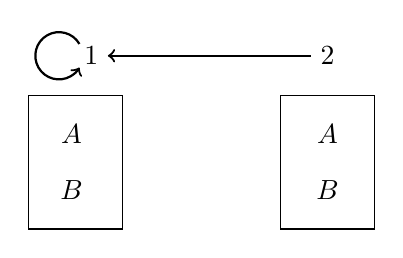
\begin{tikzpicture}
		\node (atom1) at (0,1) {1};
		\node (atom2) at (3,1) {2};
		\node (atom3) at (-0.25,0) {$A$};
		\node (atom4) at (3,0) {$\enot A$};
		\node (atom5) at (-0.25,-0.7) {$\enot B$};
		\node (atom6) at (3,-0.7) {$B$};
		\draw[->, thick] (atom1)+(-0.15,0.15) arc (-330:-30:.3);
		%\draw[->, thick] (atom2)+(0.15,-0.15) arc (-150:150:.3); 
		\draw[<-, thick] (atom1) -- (atom2);
		\draw (-0.8,-1.2) rectangle (0.4,0.5);
		\draw (2.4,-1.2) rectangle (3.6,0.5);
	\end{tikzpicture}
\end{center}
Qual a interpretação deste diagrama? Ele contém apenas dois mundos, 1 e 2. As setas entre os mundos indicam a relação de acessibilidade. Os mundos 1 e 2 acessam o mundo 1, mas nem 1 nem 2 acessam o mundo 2. As caixas em cada mundo nos permitem saber quais sentenças atômicas são verdadeiras em cada mundo: `$A$' é verdadeira em 1 mas  falsa em 2; `$B$' é falsa em 1 mas verdadeira em 2. Você só pode escrever uma sentença atômica ou a negação dela  em cada uma dessas caixas. A partir daí, podemos descobrir facilmente quais são os valores de verdade das sentenças complexas em cada mundo. Por exemplo, nessa interpretação, todas as sentenças a seguir são verdadeiras em $w_1$: 
 
\begin{itemize}
	\item[]$A\eand\enot B$, \,\,\, $B\eif A$, \,\,\, $\ediamond A$, \,\,\, $\ebox\enot B$
\end{itemize}
Se você não gosta de pensar através de diagramas, pode então expressar essa mesma interpretação assim:
\begin{itemize}
	\item[$W$:]$1,2$
	\item[$R$:]$\langle 1,1\rangle, \langle 2,1\rangle$
	\item[]$\nu_{1}(A)=V, \nu_{2}(B)=F, \nu_{2}(A)=F, \nu_{2}(B)=V$
\end{itemize}
Você terá a chance de preparar suas próprias interpretações 
em breve, quando começarmos a olhar para \emph{contrainterpretações}.


%%%\section{Uma semântica para o Sistema  K}

\section{Uma semântica para o sistema \mlK}
\label{SemanticsK}

Agora podemos estender todos os conceitos semânticos da  LVF para cobrir também a LM:
\factoidbox{
	\begin{itemize}
		\item  $\metav{A}_1,\metav{A}_2, \dots \metav{A}_n\therefore\metav{C}$ é válido em \mlK{} se e somente se não há nenhum mundo em nenhuma interpretação em que $\metav{A}_1,\metav{A}_2, \dots \metav{A}_n$ são todas verdadeiras e $\metav{C}$ é falsa.

		\item $\metav{A}$ é uma validade lógica em \mlK{} se e somente se $\metav{A}$ é verdadeira em todos os mundos e em todas as interpretações.

		\item $\metav{A}$ é uma contradição em \mlK{} se e somente se $\metav{A}$ é falsa em todos os mundos e em todas as interpretações.

		\item $\metav{A}_1,\metav{A}_2, \dots \metav{A}_n$ são compatíveis em \mlK{} se e somente se há algum mundo em alguma interpretação em que todas são verdadeiras.
	\end{itemize}
}


 Também podemos estender o uso de `$\entails$'. Para isso, precisamos adicionar subscritos da mesma forma como fizemos com `$\proves$'. Assim, quando quisermos dizer que o argumento $\metav{A}_1,\metav{A}_2, \dots \metav{A}_n\therefore\metav{C}$  é válido em \mlK, escreveremos: $\metav{A}_1,\metav{A}_2, \dots \metav{A}_n\entails_\mlK\metav{C}$. 


Para se ter uma ideia melhor desses conceitos semânticos, vejamos algumas contrainterpretações. Considere a seguinte afirmação (falsa):

\begin{itemize}
	\item[]
	      \begin{itemize}
		      \item[]$\enot A\entails_\mlK \enot \ediamond A$
	      \end{itemize}
\end{itemize}
Como obter uma contrainterpretação para essa afirmação? Precisamos construir uma interpretação na qual `$\enot A$' é verdadeira em algum mundo $w$, e `$\enot\ediamond A$ é falsa   nesse mundo $w$. Aqui está uma dessas interpretações, apresentada em um diagrama:
\begin{center}
	\begin{tikzpicture}
		\node (atom1) at (0,1) {1};
		\node (atom2) at (3,1) {2};
		\node (atom3) at (-0.25,0) {$\enot A$};
		\node (atom4) at (3,0) {$A$};
		\draw[->, thick] (atom1) -- (atom2);
		\draw (-0.8,-0.6) rectangle (0.4,0.5);
		\draw (2.4,-0.6) rectangle (3.6,0.5);
	\end{tikzpicture}
\end{center}
É fácil ver que isso funciona como uma contrainterpretação para  $\enot A\entails_\mlK\enot\ediamond A$. Em primeiro lugar, `$\enot A$' é verdadeira no mundo $1$. 
E, em segundo lugar, como `$A$' é verdadeira em $2$ e $2$ é acessível a partir de $1$, então temos que `$\ediamond A$' é verdadeira em $1$, e consequentemente `$\enot\ediamond A$'   é falsa em $1$. 
Portanto, há algum mundo nessa interpretação onde `$\enot A$' é verdadeira e `$\enot\ediamond A$'  falsa, e, por isso,     
$\enot A\nentails_\mlK \enot \ediamond A$.


Por que escolhemos o subscrito \mlK? Existe uma relação importante entre o sistema \mlK{} e a definição de validade que acabamos de fornecer. Em particular, temos os dois resultados a seguir:
\begin{itemize}
	\item Se $\metav{A}_1,\metav{A}_2, \dots \metav{A}_n\proves_\mlK\metav{C}$, então $\metav{A}_1,\metav{A}_2, \dots \metav{A}_n\entails_\mlK\metav{C}$
	\item Se $\metav{A}_1,\metav{A}_2, \dots \metav{A}_n\entails_\mlK\metav{C}$, então $\metav{A}_1,\metav{A}_2, \dots \metav{A}_n\proves_\mlK\metav{C}$
\end{itemize}
O primeiro resultado é conhecido como \emph{correção}, pois nos diz que as regras de \mlK{} são boas e corretas: se você pode justificar um argumento fornecendo uma prova dele usando o sistema \mlK, então esse argumento é realmente válido. O segundo resultado é conhecido como    \emph{completude}, uma vez que nos diz que as regras de \mlK{} são amplas o suficiente para capturar todos os argumentos válidos: se um argumento é válido, então será possível oferecer uma prova em \mlK{} que o justifique.
 

Chamamos atenção para o fato de que uma coisa é enunciar esses resultados, outra bem diferente é prová-los. Provar os teoremas da correção e completude para os sistemas modais está fora de nossos objetivos aqui, que são meramente introdutórios. Mas podemos, pelo menos, usar essa definição semântica de validade em  \mlK{} para entender melhor o funcionamento das subprovas estritas e das regras R$\mlK$ e  \ebox I.

Em uma subprova estrita, não  é permitido fazer uso de qualquer informação que esteja fora dela, exceto o que importamos para a subprova estrita usando a regra  R$\mlK$. Se tivermos assumido ou provado $\ebox \metav{A}$, então por  R$\mlK$ podemos usar a sentença  $\metav{A}$ dentro de uma subprova estrita. E em \mlK, essa é a única maneira de importar uma sentença para dentro de uma subprova estrita.
 Portanto, tudo o que pode ser provado dentro de uma subprova estrita deve seguir a partir de uma  sentença  $\metav{A}$ onde fora da subprova estrita temos $\ebox \metav{A}$.
 Assim, seguindo o raciocínio acima, se provamos uma sentença $\metav{B}$ dentro da subprova estrita, $\metav{B}$ depende apenas da  uma sentença $\metav{A}$ onde fora da subprova estrita temos $\ebox\metav{A}$.  Nessas condições, podemos obter  $\ebox\metav{B}$,  por \ebox I.
 
  Vamos imaginar agora que estejamos raciocinando sobre o que é verdade em um mundo possível em alguma interpretação. Se sabemos que $\ebox\metav{A}$ é verdadeira em um mundo possível $w$, então sabemos que $\metav{A}$ e, consequenteme, $\metav{B}$  são verdadeiras em todos os mundos acessíveis a ele.
  Portanto, como tudo o que for provado dentro de uma subprova estrita é verdadeiro em todos os mundos possíveis acessíveis a $w$, então $\ebox\metav{B}$ é verdadeira $w$. É por isso que \ebox I é uma regra correta.

%%%%%\section{Uma semântica para o sistema T}

\section{Uma semântica para o sistema \mlT}
\label{SemanticsT}

Dissemos que o sistema \mlK{} é correto e completo em relação à definição de validade que demos acima. Mas,  o que podemos afirmar sobre os outros sistemas modais \mlT, \mlSfour{}  e \mlSfive  ? Bem, eles são todos  \emph{incorretos} com respeito a essa definição de validade. Por exemplo, todos esses sistemas permitem inferir $A$ a partir de $\ebox A$, embora  $\ebox A\nentails_\mlK A$.

Isso significa que esses sistemas são uma perda de tempo? De jeito nenhum! Significa apenas que cada um dos sistemas \mlK{}, \mlT, \mlSfour{}  e \mlSfive{} formaliza uma noção de validade diferente, $\entails_\mlK$, $\entails_\mlT$, $\entails_\mlSfour$ e $\entails_\mlSfive$, cada uma delas é correta e completa com relação ao seu respectivo sistema. Então, para lidar com os outros sistemas precisamos modificar nossa definição de `$\entails$', assim como, as definições de validade lógica, contradição e compatibilidade entre sentenças.  
É nesta tarefa que a  relação de acessibilidade mostrará sua utilidade.  

Quando introduzimos a ideia de uma relação de acessibilidade, dissemos que poderia ser qualquer relação entre mundos de que você goste:  em uma interpretação a relação de acessibilidade pode ligar todos os mundos, relacionando cada um com todos os outros; em outra interpretação ela pode separar todos os mundos, não relacionando nenhum mundo com nenhum outro. E ela pode situar-se em qualquer ponto entre esses dois extremos. É assim, com esta ampla flexibilidade, que as relações de acessibilidade funcionam em nossa definição de $\entails_\mlK$. 

Mas se quisermos, podemos colocar algumas restrições nas relações de acessibilidade que podem fazer parte das interpretações. Podemos, por exemplo, exigir que as relações de acessibilidade sejam sempre \emph{reflexivas}:

\begin{itemize}
	\item $\forall wRww$
\end{itemize}
Isto significa que todo mundo acessa ele próprio.  Com   essa restrição podemos introduzir uma nova relação de consequência, $\entails_\mlT$, como segue:
\factoidbox{
	$\metav{A}_1,\metav{A}_2, \dots \metav{A}_n\entails_\mlT \metav{C}$  se e somente se  não existe nenhum mundo em qualquer interpretação \emph{que tenha uma relação de acessibilidade reflexiva}, na qual $\metav{A}_1,\metav{A}_2, \dots \metav{A}_n$ são todas verdadeiras e $\metav{C}$ é falsa.
}
Anexamos o subscrito \mlT{}  a `$\entails$' porque verifica-se que o sistema \mlT{} é correto e completo em relação a esta nova definição de validade:
\begin{itemize}
	\item Se $\metav{A}_1,\metav{A}_2, \dots \metav{A}_n\proves_\mlT\metav{C}$, então $\metav{A}_1,\metav{A}_2, \dots \metav{A}_n\entails_\mlT\metav{C}$
	\item Se $\metav{A}_1,\metav{A}_2, \dots \metav{A}_n\entails_\mlT\metav{C}$, então $\metav{A}_1,\metav{A}_2, \dots \metav{A}_n\proves_\mlT\metav{C}$
\end{itemize}
Como antes, não provaremos os resultados de correção e completude. 

Lembramos que o sistema \mlT{} é uma extensão de \mlK{} (Seção \ref{T})  e na seção anterior apresentamos um esboço da correção da  regra \ebox I.  Agora, mostraremos  que a regra  \ebox E é correta, se a relação de acessibilidade for reflexiva.  

\factoidbox{
	\[\begin{nd}
			\have[m]{m}{\ebox \metav{A}}
			\have[\, ]{n}{\metav{A}}\boxe{m}
		\end{nd}\]
}
Para justificar a regra \ebox E, é suficiente mostrar que não existe uma  contrainterpretação para:
\[
	\ebox \metav{A}\entails_\mlT \metav{A}
\]
 
 Caso existisse,  precisaríamos construir  uma interpretação  na qual $\ebox \metav{A}$ fosse verdadeira em algum  mundo  $w$, mas $\metav{A}$ fosse falsa nesse mundo.  Neste caso teríamos:

  \begin{itemize}
	\item[(1)]  $\ebox \metav{A}$ é verdadeira em $w$   \,\,\,\,\,\,  e \,\,\,\,\,\,  (2)\, $\metav{A}$  é falsa em $w$.   
\end{itemize}
Mas, como como a relação de acessibilidade é reflexiva, $w$ acessa $w$, logo: 
\begin{itemize}
	\item[(3)]  $Rww$.
\end{itemize}
De (1) podemos concluir que $\metav{A}$ deve ser verdadeira em todos os mundos acessíveis a $w$, em particular nele próprio,  pois em (3) temos que $Rww$. Logo:
\begin{itemize}
	\item[(4)]   $\metav{A}$ é verdadeira em $w$.
\end{itemize}
De (2) e  (4) chegamos a uma contradição!  Portanto, não há uma interpretação  na qual $\ebox\metav{A}$ seja verdadeira em um dado mundo, mas  $\metav{A}$  falsa nesse mundo. Consequentemente,   $\ebox \metav{A}\entails_\mlT \metav{A}$ é válido.


%%%% \section{Uma semântica para S4}

\section{Uma semântica para o sistema \mlSfour}
\label{SemanticsS4}

De que outra forma podemos ajustar nossa definição de validade? Podemos também estipular que a relação de acessibilidade seja \emph{transitiva}:
\begin{itemize}
	\item $\forall w_1\forall w_2\forall w_3 ((Rw_1w_2 \eand Rw_2w_3)\eif Rw_1w_3)$
\end{itemize}
Isso significa que se  $w_1$ acessa $w_2$, e $w_2$ acessa $w_3$, então  $w_1$ acessa $w_3$. Ou seja, a acessibilidade entre mundos forma cadeias de acessibilidade indireta e todos os mundos nessas cadeias devem ser levados em consideração na decisão sobre se algo é possível ou não. Com essa restrição imposta  à nossa relação de acessibilidade, temos uma nova relação de consequência, $\entails_\mlSfour$, como segue:
\factoidbox{
	$\metav{A}_1,\metav{A}_2, \dots \metav{A}_n\entails_\mlSfour \metav{C}$ se e somente se não existe nenhum mundo em qualquer interpretação \emph{que tenha uma relação de acessibilidade reflexiva e transitiva}, na qual $\metav{A}_1,\metav{A}_2, \dots \metav{A}_n$ são todas verdadeiras e $\metav{C}$ é falsa
}
Anexamos o subscrito \mlSfour{}  a `$\entails$' porque verifica-se que o sistema \mlSfour{} é correto e completo em relação a esta nova definição de validade:
\begin{itemize}
	\item Se $\metav{A}_1,\metav{A}_2, \dots \metav{A}_n\proves_\mlSfour\metav{C}$, então $\metav{A}_1,\metav{A}_2, \dots \metav{A}_n\entails_\mlSfour\metav{C}$
	\item Se $\metav{A}_1,\metav{A}_2, \dots \metav{A}_n\entails_\mlSfour\metav{C}$, então $\metav{A}_1,\metav{A}_2, \dots \metav{A}_n\proves_\mlSfour\metav{C}$
\end{itemize}
Como antes, não provaremos esses resultados. Daremos apenas uma ideia de como mostrar que as regras de inferência de \mlSfour{} são corretas.

Ora, vimos na Seção \ref{S4} que o sistema \mlSfour{} é uma extensão de \mlT{} e já mostramos na seção anterior que  a regra  \ebox E é correta quando a relação de acessibilidade é reflexiva; e é relativamente fácil justificar  a regra  R$\mathbf{4}$, se a relação de acessibilidade for transitiva.

 
\factoidbox{
	\[\begin{nd}
			\have[m]{m}{\ebox\metav{A}}
			\open
			\hypo[\ ]{k}{\ebox}
			\have[\ ]{n}{\ebox\metav{A}}\rfour{m}
		\end{nd}\]
}

Lembramos que a ideia por trás das subprovas estritas é que elas são maneiras de provar coisas que devem ser verdadeiras em todos os mundos acessíveis. Assim, a regra R$\mathbf{4}$  significa que sempre que $\ebox \metav{A}$ for verdadeira em um mundo, $\ebox \metav{A}$ também deve ser verdadeira  em todos os mundos acessíveis  a este mundo. Logo, devemos ter $\ebox\metav{A} \entails_\mlSfour \ebox\ebox\metav{A}$.

Para constatar isso, tente construir uma contrainterpretação para esta afirmação:
\begin{itemize}
	\item[]$\ebox\metav{A} \entails_\mlSfour \ebox \ebox \metav{A}$
\end{itemize}
 

 Precisaríamos construir uma interpretação na qual $\ebox\metav{A}$ seja verdadeira em um dado mundo  $w_1$, mas  $\ebox \ebox \metav{A}$  falsa nesse mundo. Assim teríamos: 
 \begin{itemize}
	\item[(1)]  $\ebox\metav{A}$ é verdadeira em $w_1$ \,\,\,\,\,\,  e \,\,\,\,\,\,  (2)\, $\ebox \ebox \metav{A}$  é  falsa em  $w_1$.
\end{itemize} 
De (2) se segue que $w_1$ deve acessar algum mundo $w_2$, no qual $\ebox\metav{A}$ é falsa.  Logo, existe um $w_2$ tal que: 
\begin{itemize}
	\item[(3)]  $Rw_1w_2$  \,\,\,\,\,\,  e \,\,\,\,\,\,  (4)\, $\ebox\metav{A}$ é falsa em $w_2$.
\end{itemize}
De (4) podemos concluir que $w_2$ deve acessar algum mundo  $w_3$, no qual $\metav{A}$ é falsa. 
Logo, existe um $w_3$ tal que:
\begin{itemize}
	\item[(5)]  $Rw_2w_3$  \,\,\,\,\,\, e  \,\,\,\,\,\, (6)\,  $\metav{A}$ é falsa em $w_3$.
\end{itemize}
Como a relação de acessibilidade é transitiva, de (3) e (5) temo que $w_1$ acessa $w_3$, isto é: 
\begin{itemize}
	\item[(7)]  $Rw_1w_3$.
\end{itemize}
Mas,  de (1) podemos concluir que  $\metav{A}$  é verdadeira em todo mudo acessível a $w_1$, em particular, verdadeira em $w_3$. Assim: 
\begin{itemize}
	\item[(8)]  $\metav{A}$  é verdadeira em $w_3$.
\end{itemize}
 De (6) e (8), temos que  $\metav{A}$ é verdadeira e falsa em $w_3$. Contradição!  
  

Portanto, não há uma interpretação  na qual $\ebox\metav{A}$ seja verdadeira em um dado mundo, mas  $\ebox \ebox \metav{A}$  falsa nesse mundo. Consequentemente,  $\ebox\metav{A} \entails_\mlSfour \ebox\ebox\metav{A}$ é válido.


%%%% \section{Uma semântica para S5}
\section{Uma semântica para o sistema \mlSfive}
\label{SemanticsS5}

Vamos acrescentar mais uma restrição à relação de acessibilidade. Desta vez, impor que a relação de acessibilidade seja também \emph{simétrica}:
\begin{itemize}
	\item $\forall w_1\forall w_2(Rw_1w_2 \eif Rw_2w_1)$
\end{itemize}
Isto significa que se  $w_1$ acessa $w_2$, então $w_2$ acessa  $w_1$. Os lógicos chamam uma relação que é reflexiva, simétrica e transitiva de \emph{relação de equivalência}. Agora podemos  definir uma nova relação de consequência, $\entails_\mlSfive $, como segue:

\factoidbox{
	$\metav{A}_1,\metav{A}_2, \dots \metav{A}_n\entails_\mlSfive  \metav{C}$ se e somente se  não existe nenhum mundo em qualquer interpretação \emph{cuja relação de acessibilidade seja uma relação de equivalência}, na qual $\metav{A}_1,\metav{A}_2, \dots \metav{A}_n$ são todas verdadeiras e $\metav{C}$ é falsa.
}
Anexamos o subscrito \mlSfive{} a `$\entails$' porque  o sistema \mlSfive{} é correto e completo em relação a esta nova definição de validade:

\begin{itemize}
	\item Se $\metav{A}_1,\metav{A}_2, \dots \metav{A}_n\proves_\mlSfive \metav{C}$, então $\metav{A}_1,\metav{A}_2, \dots \metav{A}_n\entails_\mlSfive \metav{C}$
	\item Se $\metav{A}_1,\metav{A}_2, \dots \metav{A}_n\entails_\mlSfive \metav{C}$, então $\metav{A}_1,\metav{A}_2, \dots \metav{A}_n\proves_\mlSfive \metav{C}$
\end{itemize}
Aqui também não provaremos esses resultados.  No entanto, é relativamente fácil  justificar  a  regra   R$\mathbf{5}$,  se a relação de acessibilidade for uma relação de equivalência.

\factoidbox{
	\[\begin{nd}
			\have[m]{m}{\enot\ebox \metav{A}}
			\open
			\hypo[\ ]{k}{\ebox}
			\have[\, ]{n}{\enot\ebox\metav{A}}\rfive{m}
		\end{nd}\]
}


Essa regra diz que se $\metav{A}$ não é necessária, ou seja, falsa em algum mundo acessível, também não é necessária em qualquer mundo possível acessível. 
 Temos então $\enot\ebox \metav{A} \entails_\mlSfive \ebox\enot\ebox \metav{A}$.

Para constatar isso, tente construir uma contrainterpretação para esta afirmação:
\[
	\enot\ebox\metav{A} \entails_\mlSfive  \ebox \enot\ebox \metav{A}
\]
 
 

Precisaríamos construir uma interpretação  na qual  $\enot\ebox\metav{A}$ é verdadeira em um mundo $w_1$, mas  $\ebox \enot\ebox \metav{A}$  é falsa nesse mundo. Assim teríamos:

  \begin{itemize}
	\item[(1)]  $\enot\ebox\metav{A}$ é verdadeira em $w_1$   \,\,\,\,\,\,  e \,\,\,\,\,\,  (2)\, $\ebox \enot\ebox \metav{A}$  é falsa em $w_1$.   
\end{itemize} 
De (1) se segue que $\ebox\metav{A}$ é falsa em  $w_1$. Assim, $w_1$  deve acessar algum mundo $w_2$, no qual $\metav{A}$ é falsa. Logo existe um mundo $w_2$ tal que:
 \begin{itemize}
	\item[(3)]  $Rw_1w_2$      \,\,\,\,\,\,  e \,\,\,\,\,\,  (4)\, $\metav{A}$ é falsa em $w_2$.  
\end{itemize} 
De (2), podemos concluir que $w_1$ deve acessar algum mundo $w_3$, no qual $\enot\ebox \metav{A}$ é falsa. Logo,  existe um mundo $w_3$ tal que:
 \begin{itemize}
	\item[(5)]  $Rw_1w_3$   \,\,\,\,\,\,  e \,\,\,\,\,\,  (6)\, $\enot\ebox \metav{A}$ é falsa em $w_3$.  
\end{itemize} 
Como agora temos a restrição que a relação de acessibilidade é uma relação de equivalência e, portanto, simétrica,  de (5) podemos inferir que $w_3$ acessa  $w_1$. Ou seja:
\begin{itemize}
	\item[(7)]   $Rw_3w_1$. 
\end{itemize}
Como  $R$ é uma relação de equivalência,  $R$ é transitiva. Assim de (7) e (3) podemos inferir  que $w_3$ acessa $w_2$. Assim,   temos:
 \begin{itemize}
	\item[(8)]   $Rw_3w_2$     
\end{itemize} 
 Mas, de (6) se segue que $\ebox \metav{A}$   é verdadeira em $w_3$ e consequentemente, $\metav{A}$ é verdadeira em todos os mundos que $w_3$ acessa, em particular $w_2$, pois em (8) temos que $Rw_3w_2$. Logo:
 \begin{itemize}
	\item[(9)]  $\metav{A}$ é verdadeira em $w_2$.        
\end{itemize} 
De (4)  e (9) chegamos à uma Contradição!
Portanto, não há uma interpretação  na qual $\enot\ebox\metav{A}$ seja verdadeira em um dado mundo, mas  $\ebox \enot\ebox \metav{A}$  falsa nesse mundo. Consequentemente,  $\enot\ebox \metav{A} \entails_\mlSfive \ebox\enot\ebox \metav{A}$ é válido. \\

Na definição de  $\entails_\mlSfive $, estipulamos que a relação de acessibilidade deve ser uma relação de equivalência. Mas acontece que há outra maneira de obter uma noção de validade adequada para \mlSfive. Em vez de estipular que a relação de acessibilidade seja uma relação de equivalência, podemos estipular que seja uma relação \emph{universal}:
\begin{itemize}
	\item $\forall w_1\forall w_2Rw_1w_2$
\end{itemize}
Isto significa  que todo mundo acessa todo mundo. Usando essa restrição na relação de acessibilidade, poderíamos ter definido  $\entails_\mlSfive $ assim:\factoidbox{
	$\metav{A}_1,\metav{A}_2, \dots \metav{A}_n\entails_\mlSfive  \metav{C}$ se e somente se  não existe nenhum mundo em qualquer interpretação  \emph{que tenha uma relação de acessibilidade universal}, na qual $\metav{A}_1,\metav{A}_2, \dots \metav{A}_n$ são todas verdadeiras e $\metav{C}$ é falsa.
}
Se definíssemos $\entails_\mlSfive $ assim, ainda obteríamos os mesmos resultados de correção e completude para \mlSfive{}. O que isso nos diz? Isso significa que o sistema \mlSfive{} é aquele que formaliza as noções de necessidade e possibilidade absolutas, nas quais ser possível é ocorrer em algum mundo qualquer e ser necessário é ocorrer em todos os mundos. Todos os outros sistemas (\mlK{}, \mlT{} e \mlSfour) representam algum grau de relativização destas noções de necessidade e possibilidade.
 Além disso, a maioria dos filósofos assume que as noções de necessidade com as quais estão mais preocupados, como a  \emph{necessidade lógica} e a \emph{necessidade metafísica}, são exatamente desse tipo. Portanto, \mlSfive{} é o sistema modal que a maioria dos filósofos usa na maior parte do tempo.
 

\practiceproblems

\problempart
Apresente contrainterpretações para as quatro seguintes afirmações falsas:
\begin{earg}
	\item $\enot P \entails_\mlK \enot\ediamond P$
	\item $\ebox(P \eor Q)\entails_\mlK \ebox P \eor \ebox Q$
	\item $\entails_\mlK \enot \ebox (A\eand \enot A)$
	\item $\ebox A\entails_\mlK A$
\end{earg}

\problempart
Apresente contrainterpretações para as duas seguintes afirmações falsas:
\begin{earg}
	\item $\ebox (M\eif O),\ediamond M\entails_\mlT O$
	\item $\ebox A\entails_\mlT \ebox \ebox A$
\end{earg}

\problempart
Apresente contrainterpretações para as duas seguintes afirmações falsas:
\begin{earg}
	\item $\ediamond A\entails_\mlSfour \ebox\ediamond A$
	\item $\ediamond A, \ebox (\ediamond A \eif B)\entails_\mlSfour\ebox B$
\end{earg}

\section*{Leitura adicional}

A lógica modal é um grande subcampo da lógica. Nós apenas arranhamos a superfície. Se você quiser aprender mais sobre lógica modal, aqui estão alguns livros que você pode consultar:

\begin{itemize}
	\item Hughes, G. E., \& Cresswell, M. J. (1996). \emph{A New Introduction to Modal Logic}, Oxford: Routledge.
	\item Priest, G. (2008). \emph{An Introduction to Non-Classical Logic}, 2nd ed., Cambridge: Cambridge University Press.
	\item Garson, J. W. (2013). \emph{Modal Logic for Philosophers}, 2nd ed., Cambridge: Cambridge University Press.
\end{itemize}

Nenhum desses autores formula seus sistemas de provas modais da mesma forma que nós, mas a formulação mais próxima é dada por Garson. 






